\documentclass[a4paper, 11pt]{article}
\usepackage{geometry}
\geometry{letterpaper, margin=1in}
\usepackage{amsmath}
\usepackage{amssymb}  
\usepackage{amsthm}
\usepackage{ulem} 
\usepackage{graphicx}
\graphicspath{ {images/} }

\begin{document}
%Header-Make sure you update this information!!!!
\noindent
\large\textbf{Complex Analysis - MTH 483} \hfill \textbf{John Waczak} \\
\normalsize Day 2 \hfill  Date: \today \\


\section*{Polar Coordinates}
If we have a complex number $z=x + iy$ we can also write this as $z= re^{i\phi}$. What are the $r$ and the $\phi$? $r$ is the distance to the origin $r=\sqrt{x^2+y^2}$ and $e^{i\phi} = \cos\phi + i\sin\phi$. We call $\phi$ the argument. 

Some nice properties:
	\begin{align}
		e^{i(\phi_1+\phi_2)} &= e^{i\phi_1}\cdot e^{i\phi_2} \\ 
		e^{i\cdot 0} &= 1 \\
		e^{-i\phi} &= \frac{1}{e^{i\phi}} \\
		|e^{i\phi}|&= 1 \\
		e^{i\phi+2\pi n} &= e^{i\phi} \\ 
		\frac{d}{d\phi}e^{i\phi} &= ie^{i\phi}
	\end{align}

Most can be proven by sine and cosine properties. (3) follows from (1) and (2). Others are pretty easy. Let's focus on (1):
	\begin{align*}
		e^{i(\phi_1+\phi_2)} &= cos(\phi_1+\phi_2)+i\sin(\phi_1+\phi_2) \\ 
		 &= \cos\phi_1\cos\phi_2 - \sin\phi_1\sin\phi_2 +i(\cos\phi_1\sin\phi_2+\sin\phi_1\cos\phi_2) \\ 
		 &= (\cos\phi_1+i\sin\phi_1)\cdot(\cos\phi_2+i\sin\phi_2) \\
		 &\equiv e^{i\phi_1}e^{i\phi_2} \quad \qed
	\end{align*}

The more interesting way is to go in reverse to deduce the trig identities using Taylor expansions for our functions:
	\begin{align*}
		e^{iz}e^{iw} &= \sum_{k=0}^\infty \frac{z^k}{k!}\sum_{n=0}^\infty \frac{w^k}{k!} \\ 
		&= \sum_{\ell =0}^\infty \frac{(z+w)^\ell}{\ell!} \\ 
		\text{Take: }& z=i\phi_1, w=i\phi_2
	\end{align*}
	
This is more logical because we don't have a definition of exponent of a complex number algebraically... that doesn't make much sense. So if we accept that Taylor series over the field $\mathbb{C}$ then we get these properties as a result. \\

\noindent Now let's check (6) with the fact that derivatives apply linearly to real and imaginary part. 
	\begin{align*}
		\frac{d}{d\phi}e^{i\phi} &= \frac{d}{d\phi}(\cos\phi + i\sin\phi) \\ 
			&= -\sin\phi + i\cos\phi \\ 
			&= i(\cos\phi-\frac{1}{i}\sin\phi) \\ 
			&= i(\cos\phi + i\sin\phi) \\ 
			&= ie^{i\phi}
	\end{align*}

\section*{Euler's Identity}
When you define $e^z$ as a power series you can prove Euler's Identity using Taylor expansions. In general the fancy formula is:
	\begin{equation}
		e^{i\phi}= \cos\phi + i\sin\phi
	\end{equation}
	
\noindent The very famous version is take $\phi = \pi$. 
	\begin{equation}
		e^{i\pi}+1 = 0
	\end{equation}

\noindent What this is really saying is that the sum $\sum_{n=0}^\infty (i\pi)^n/n! = -1$. You can check this with a computer. 

\section*{Transferring between coordinate systems}
Exmaple: \textit{Write $3e^{i\pi/4}$ in cart. coords.}
	\begin{align*}
		3e^{i\pi/4} &= 3(\cos(\phi/4)+i\sin(\pi/4)) \\ 
			& \frac{3\sqrt{2}}{2}(1+i)
	\end{align*}
	
\noindent Example: \textit{Write $z=1+i\sqrt{3}$ in polar coords.}
	\begin{align*}
		1+i\sqrt{3} &= 2(\frac{1}{2}+i\frac{\sqrt{3}}{2}) \\ 
			&= 2(\cos(\pi/3)+i\sin(\pi/3)) \\
			&= 2e^{i\pi/3}
	\end{align*}

\noindent Polar coordinates are super handy when we want to raise some $z$ to a power. 
	\begin{align*}
		(1+i\sqrt{3})^{10} &\text{ don't use binomial theorem!} \\ 
			&= (2e^{i\pi/3})^10 \\ 
			&= 2^{10}e^{i\frac{10\pi}{3}} \\ 
			&= 2^{10}e^{i\frac{4\pi}{3}} \\ 
			&= 2^{10}(-\frac{1}{2}-\frac{i\sqrt{3}}{2}) \\ 
			&= -2^9(-1-i\sqrt{3})
	\end{align*}


\section*{Roots of Unity} 
\textbf{Definition:} A \textit{n-root} of unity is a number $\in\mathbb{C}$ is a number $\zeta$ satisfying:
	\begin{align*}
		\zeta^n = 1
	\end{align*}
\noindent Where n is a positive integer. If n is the smallest number for which $\zeta^n=1$ then we say $\zeta$ is a \textit{primitive} root of unity. \\

\noindent Example: $1^1 = 1$ so 1 is prim first root of unity. $(-1)^2 = 1$ so $-1$ is a 2nd primitive root of unity. $i^4 = 1$ so i is a primitive fourth root of unity (so is -i). These lie on the unit circle and alway form a perfect n-gon. \\

\noindent Since $1^4 = 1$ and $(-1)^4=1$ and $(\pm i)^4 = 1$ are the fourth roots of unity (only $\pm i$ are primitive fourth roots). In general the n-th roots of unity are precisely the roots of the polynomial $f(x) = x^n -1$. By \textbf{Fundamental theorem of Algebra} there are at most n roots for a polynomial over any field i.e. the degree of the polynomial is maximum number of roots. Thus there are at most n roots of unity.\\

\noindent We would like to know if there are \textit{exactly} n roots... So far it seems like there are always n roots. In fact, using polar coordinates we can show that there are always exactly n nth-roots of unity namely:
	\begin{eqnarray}
		u_n=e^{i\frac{2\pi k}{n}} \quad k\in[1, ... , n] 
	\end{eqnarray}
\noindent Note that 1 is \textit{always} an nth-root of unity. These numbers form a regular n-gon around unit circle. 
	\begin{figure}[!hbt]
		\centering
		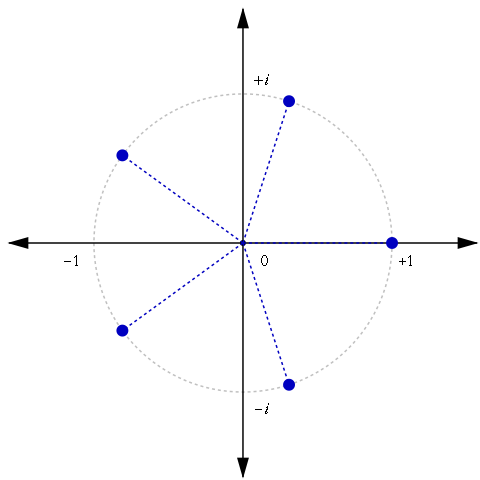
\includegraphics[width=0.4\columnwidth]{rootsOfUnity}
		\caption{5th roots of unity (regular pentagon)}
	\end{figure}











\end{document}